% 导言区
\documentclass{article}
%\documentclass{paper}

\usepackage{ctex}
\usepackage{amsmath}
\usepackage{graphicx}
\usepackage{bbding}
\usepackage{multirow}
\usepackage{listings}



\graphicspath{{figs/}}

\title{\heiti 第一次作业}
\author{\kaishu 宋晓宇}
\date{}
\newcommand{\bs}{\boldsymbol}
\newcommand{\p}[1]{\includegraphics[width=0.7\textwidth]{#1}}

% 正文区(文稿区)
\begin{document}
	\maketitle
	\section*{1.}
	\subsection*{a)}
	$S_1\cup S_2$不是凸集.
	
	反例:若$S_1=\{(x,y)|(x+2)^2+y^2\leq 1\}$,$S_2=\{(x,y)|(x-2)^2+y^2\leq 1\}$,取$x=(-2, 0)\in S_1$,$y=(2, 0)\in S_2$,即$x,y\in S_1\cup S_2$,取$z=0.5x+0.5y=(0, 0)$,则$z\notin S_1\cup S_2$,因此$S_1\cup S_2$不是凸集.
	\subsection*{b)}
	$S_1+S_2$是凸集.
	
	证明:对于任意的$z_1,z_2\in S_1+S_2$,存在$x_1,x_2\in S_1, y_1,y_2\in S_2$,使得$z_1=x_1+y_1, z_2=x_2+y_2$,则对于任意的$\beta\in (0,1)$,$\beta z_1+(1-\beta)z_2=\beta(x_1+y_1)+(1-\beta)(x_2+y_2)=(\beta x_1+(1-\beta)x_2)+(\beta y_1+(1-\beta)y_2)$;由于$S_1$,$S_2$是凸集,$\beta x_1+(1-\beta)x_2\in S_1$,$\beta y_1+(1-\beta)y_2\in S_2$,因此$(\beta x_1+(1-\beta)x_2)+(\beta y_1+(1-\beta)y_2)\in S_1+S_2$,即$\beta z_1+(1-\beta)z_2\in S_1+S_2$,因此$S_1+S_2$是凸集.
	
	\subsection*{c)}
	$S_1-S_2$是凸集.
	
	证明:对于任意的$z_1,z_2\in S_1-S_2$,存在$x_1,x_2\in S_1, y_1,y_2\in S_2$,使得$z_1=x_1-y_1, z_2=x_2-y_2$,则对于任意的$\beta\in (0,1)$,$\beta z_1+(1-\beta)z_2=\beta(x_1-y_1)+(1-\beta)(x_2-y_2)=(\beta x_1+(1-\beta)x_2)-(\beta y_1+(1-\beta)y_2)$;由于$S_1$,$S_2$是凸集,$\beta x_1+(1-\beta)x_2\in S_1$,$\beta y_1+(1-\beta)y_2\in S_2$,因此$(\beta x_1+(1-\beta)x_2)-(\beta y_1+(1-\beta)y_2)\in S_1-S_2$,即$\beta z_1+(1-\beta)z_2\in S_1-S_2$,因此$S_1-S_2$是凸集.
	\section*{2.}
	\subsection*{a)}
	$S$不是凸集.
	
	理由:取$z_1=(-4,-2), z_2=(4,0)$,则$z_1\in S, z_2\in S$,由于$0.5z_1+0.5z_2=(0, -1)\notin S$,所以$S$不是凸集.

	\subsection*{b)}
	
	$S$是凸集.
	
	理由:如图.
	
%	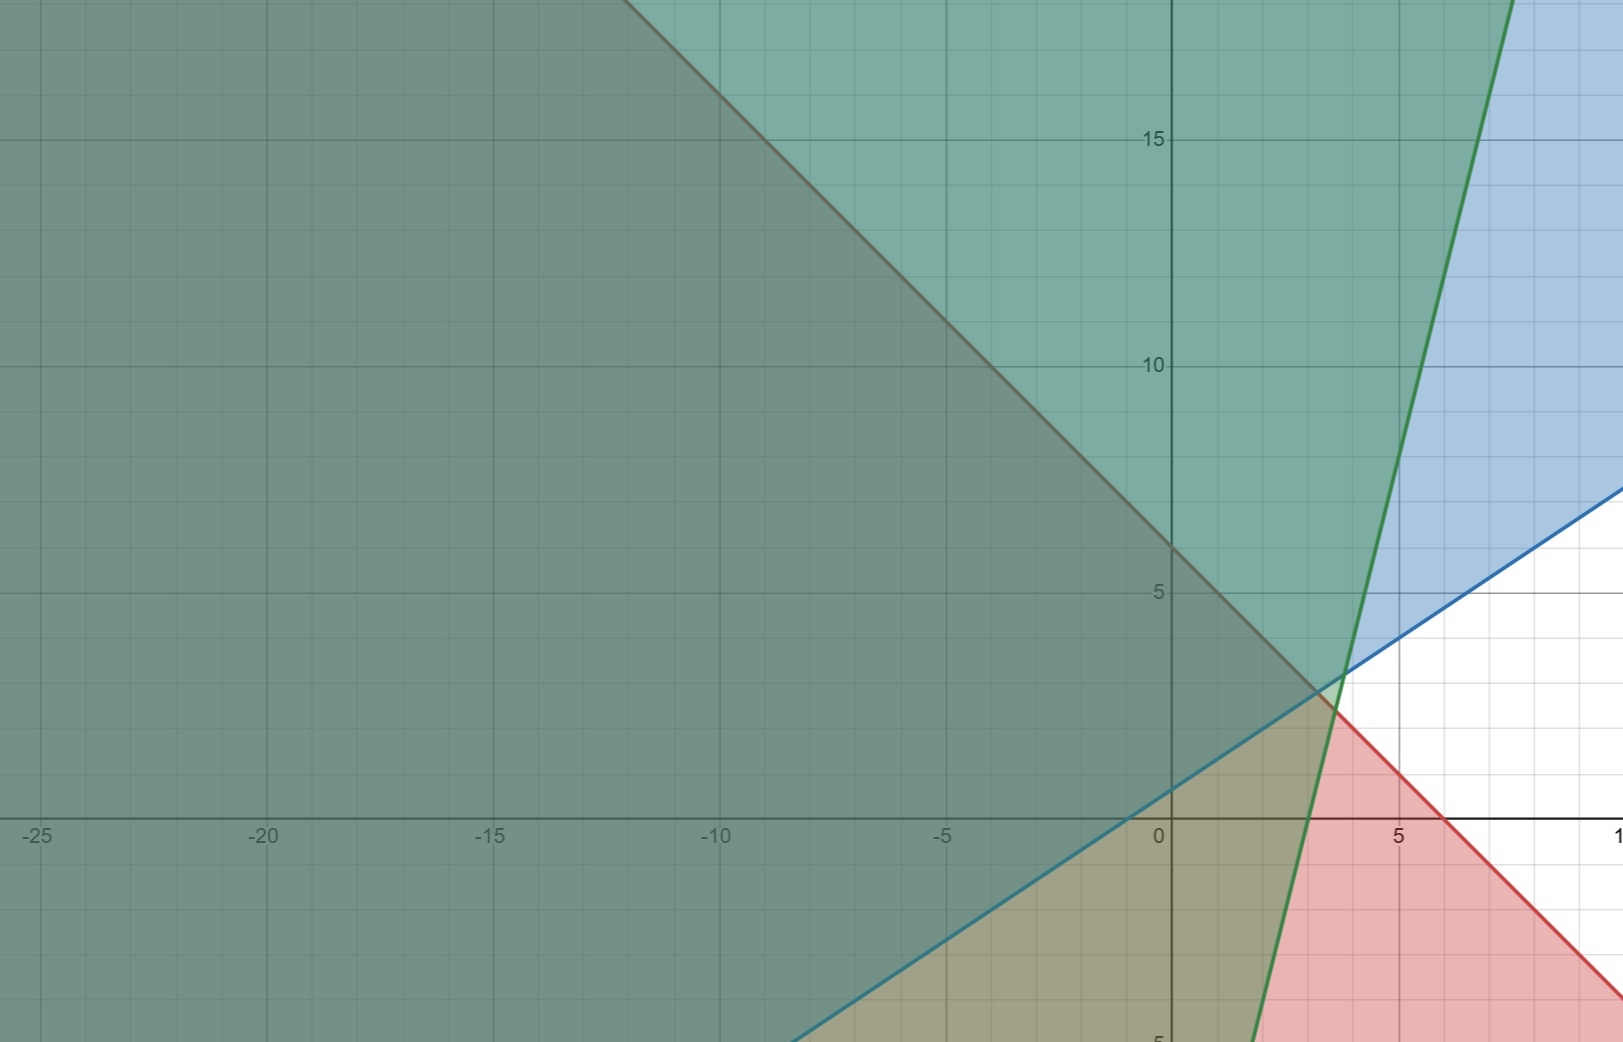
\includegraphics[width=0.9\textwidth]{2-b}
	\p{2-b}
	\subsection*{c)}
	
	$S$是凸集.
	
	理由:如图.
	
	\p{2-c}
	
	\subsection*{d)}
	
	$S$不是凸集.
	
	理由:取$x_1=-2\in S, x_2=2\in S$,则$0.5x_1+0.5x_2=0\notin S$,因此$S$不是凸集.

	\section*{3.}
	
	\subsection*{a)}
	
	$g(x)$是凸函数.
	
	证明:$\forall \lambda \in (0,1), g(\lambda x+(1-\lambda)y)=max\{f_1(\lambda x+(1-\lambda)y),\cdots, f_m(\lambda x+(1-\lambda)y)\}\leq max\{\lambda f_1(x)+(1-\lambda)f_1(y),\cdots, \lambda f_m(x)+(1-\lambda)f_m(y)\}\leq \lambda max\{f_1(x),\cdots,f_m(x)\}+(1-\lambda)max\{f_1(y),\cdots,f_m(y)\}\leq \lambda g(x)+(1-\lambda)g(y)$,因此$g(x)$是凸函数.
	\subsection*{b)}
	$g(x)$不是凸函数.
	
	反例:令$f_1(x)=(x+1)^2, f_2(x)=(x-1)^2$,则$g(-1)=0, g(1)=0$,又$g(0)=1$,因此$g(0.5\cdot (-1)+0.5\cdot 1) > 0.5g(-1)+0.5g(1)$,因此$g(x)$不是凸函数.
	
	\subsection*{c)}
	
	$g(x)$是凸函数.

	证明:令$f(x)=xlog(x)$,易知$f(x)$是凸函数,$g(x)=\sum^n_{i=1}f(x_i)$,因此对于任意的$\lambda \in (0,1)$,有$g(\lambda x+(1-\lambda)y)=\sum^n_{i=1}f(\lambda x+(1-\lambda)y)\leq\sum^n_{i=1}(\lambda f(x)+(1-\lambda)f(y))=\lambda g(x)+(1-\lambda)g(y)$因此$g(x)$是凸函数.
	
	\subsection*{d)}
	
	$g(x)$不是凸函数.
	
	证明:$g(0.5\cdot (-1.5)+0.5\cdot 1.5)=g(0)=0$,而$0.5g(-1.5)+0.5g(1.5)=-1$,因此$g(0.5\cdot (-1.5)+0.5\cdot 1.5)>0.5g(-1.5)+0.5g(1.5)$,因此$g(x)$不是凸函数.

	\subsection*{e)}
	
	$g(x)$是凸函数.
	
	证明:不妨设x,y满足$x_1 \geq x_2 \geq \cdots \geq x_n$,$y_1 \geq y_2 \geq \cdots \geq y_n$,此时$g(\lambda x+(1-\lambda)y)=\lambda g(x)+(1-\lambda)g(y)$. 当x,y分量顺序任意打乱得到$x^\prime ,y^\prime$时,$g(\lambda x^\prime+(1-\lambda)y^\prime)\leq g(\lambda x+(1-\lambda)y)$,因此$g(\lambda x^\prime+(1-\lambda)y^\prime)\leq \lambda g(x)+(1-\lambda)g(y)=\lambda g(x^\prime)+(1-\lambda)g(y^\prime)$,$g(x)$是凸函数.
	
	\subsection*{f)}
	
	$g(x)$是凸函数.
	
	证明:$g(x)$二次可微,且$\nabla^2g(x)=2>0$,因此$g(x)$是凸函数.
	
	
	\section*{4.}
	
	\subsection*{a)}
	
	化为标准型:$Max\ z=2x_1^\prime+x_2-2x_3^\prime+2x_4,\ s.t. \begin{cases}
		x_1^\prime+x_2+x_3^\prime-x_4=4 \\
		x_1^\prime+x_2-x_3^\prime+x_4+x_5=6\\
		x_1^\prime, x_2, x_3^\prime, x_4, x_5 \geq 0
	\end{cases}$.
	
	$A=\begin{bmatrix} 1 & 1 & 1 & -1 & 0 \\ 1 & 1 & -1 & 1 & 1\end{bmatrix}$,$b=\begin{bmatrix} 4 \\ 6\end{bmatrix}$,$c=(2,1,-2,2,0)$.
	
	令$B=[P_1,P_3]=\begin{bmatrix} 1 & 1\\ 1&-1 \end{bmatrix}$,则$x_B=B^{-1}b=\begin{bmatrix} 5 \\ -1\end{bmatrix}$,$x_B$出现负数,不是可行解.
	
	令$B=[P_1,P_5]=\begin{bmatrix} 1 & 0\\ 1&1 \end{bmatrix}$,则$x_B=B^{-1}b=\begin{bmatrix} 5 \\ 1\end{bmatrix}$,$x_B$是最优可行解,代入可得$z=12$.	
	
	\subsection*{b)}

	化为标准型:$Max\ z=-2x_1+x_2^\prime-3x_3-x^\prime_4+x_5,\ s.t. \begin{cases}
	x_1-x_2^\prime+x_3+x_4^\prime-x_5+x_6=7 \\
	2x_1+3x_2^\prime+5x_3=-8 \\
	x_1-2x_3+2x_4^\prime-2x_5-x_7=1 \\
	x_1, x_2^\prime, x_3, x_4^\prime, x_5, x_6, x_7 \geq 0
    \end{cases}$.
    由于$x_1, x_2^\prime, x_3 \geq 0$, $2x_1+3x_2^\prime+5x_3$不可能等于$-8$,此问题无解.
	\section*{5.}
	
	\subsection*{a)}
	
	如图,可行域为空集,问题无解。
	
	\p{5-a}
	
	\subsection*{b)}
	
	如图.
	
	\p{5-b}
	
	梯度方向为$(-1,3)$. 存在无界最优解.
	\section*{6.}
	
	\subsection*{(1)}
	
	令$x_1, x_2$为基变量,$x_3, x_4,x_5$为非基变量,求得一个基本解为$(\frac{14}{3},-\frac{1}{3},0,0,0)$.
	
	\subsection*{(2)}
	
	令$x_1, x_4$为基变量,$x_2, x_3,x_5$为非基变量,求得一个基本解为$(3,0,0,-1,0)$.
	
	
	\subsection*{(3)}
	
	令$x_4, x_5$为基变量,$x_1, x_2,x_3$为非基变量,求得一个基本解为$(0,0,0,-1,3)$.
	
	\section*{7.}
	
	\subsection*{(1)}
	
	令$x_1, x_2$为基变量,$x_3, x_4$为非基变量,$B=\begin{bmatrix} 2 & 4 \\ 4 & 10\end{bmatrix}$,$B^{-1}=\begin{bmatrix} \frac{5}{2} & -1 \\ -1 & \frac{1}{2}\end{bmatrix}$,$N=\begin{bmatrix} 2 & 2 \\ 6 & 8\end{bmatrix}$,$x_B=(-2,2)^T$,$x_N=(0,0)^T$,$x^{(1)}=(-2,2,0,0)^T$.
	
	\subsection*{(2)}
	
	令$x_1, x_3$为基变量,$x_2, x_4$为非基变量,$B=\begin{bmatrix} 2 & 2 \\ 4 & 6\end{bmatrix}$,$B^{-1}=\begin{bmatrix} \frac{3}{2} & -\frac{1}{2} \\ -1 & \frac{1}{2}\end{bmatrix}$,$N=\begin{bmatrix} 4 & 2 \\ 10 & 8\end{bmatrix}$,$x_B=(0,2)^T$,$x_N=(0,0)^T$,$x^{(1)}=(0,0,2,0)^T$.
	
	\section*{8.}
	
	证明:设$x=(x_1, x_2, \cdots, x_n)^T$是LP问题的一个可行解,$A=(p_1, p_2,\cdots,p_n)_{m\times n}$.
	
    充分性:
	
	设$x=(x_1,x_2,\cdots x_k, 0,\cdots,0)$是LP问题的可行解,其中前k个分量为正分量且对应的系数列向量线性无关。$r(A)=m$,$k\leq m$.
	
	若$k=m$,由定义可知$x$为基本可行解.
	
	若$k<m$,由$r(A)=m$,即$r(p_1, p_2,\cdots,p_n)=m$,则$p_1, p_2,\cdots,p_m$构成一个基矩阵,$x$是一个基本可行解.
	
	必要性:

	若可行解$x$是基本可行解。不妨设$x
	_1, \cdots, x_m$为基变量,即$(p_1,\cdots,p_m)$为基矩阵。不妨设$x_1, \cdots,x_k$为正分量,则对应的系数列向量为$p_10,\cdots,p_k$,而$(p_1,\cdots,p_k)\subset (p_1,\cdots,p_k)$且$p_1,\cdots,p_k$线性无关, 因此$p_1,\cdots,p_k$线性无关.
	
	\section*{9.}
	\subsection*{a)}
	
	化为标准型:$Max\ 6x_1+14x_2+13x_3,\ s.t. \begin{cases}
		x_1+4x_2+2x_3+x_4=48\\
		x_1+2x_2+4x_3+x_5=60\\
		x_1, x_2, x_3, x_4, x_5 \geq 0
	\end{cases} $.
	
	\begin{tabular}{|c|c|c|ccccc|c|}
		\hline
		\multirow{2}{*}{$C_B$} & \multirow{2}{*}{$x_b$} & \multirow{2}{*}{$b$} &6&14&13&0&0 & $\alpha$ \\
		\cline{4-8}
		&   & & $x_1$ & $x_1$ & $x_1$ & $x_1$ & $x_1$ & \\
		\hline
		0 & $x_4$ & 48 & 1&4&2&1&0&12\\
		0 & $x_5$ & 60 & 1&2&4&0&1&30\\
		
		\hline
		& -z & 0 & 6&14&13&0&0 & \\
		\hline
		14 & $x_2$ & 12 &0.25&1&0.5&0.25&0&24\\
		0 & $x_5$ & 36 &0.5&0&3&-0.5&1&12\\
		
		\hline
		& -z & -168 & 6&14&13&0&0 & \\
		\hline
		0 & $x_4$ & 6 & $\frac{1}{6}$&1&0&$\frac{1}{3}$&$-\frac{1}{6}$&36\\
		0 & $x_5$ & 12 & $\frac{1}{6}$&0&1&$-\frac{1}{6}$&$\frac{1}{3}$&72\\
		
		\hline
		& -z & 0 & 6&14&13&0&0 & \\
		\hline
		0 & $x_4$ & 36 & 1&6&0&2&-1&\\
		0 & $x_5$ & 6 & 0&-1&1&-0.5&0.5&\\
		
		\hline
		& -z & -294 & 0&-9&0&-7.5&-0.5 & \\
		
		\hline
	\end{tabular}
	
	$x=(36,0,6,0,0)T$,$z=294$
	
	\subsection*{b)}
	
	化为标准型:$Max\ -3x_1+2x_2+4x_3,\ s.t. \begin{cases}
		4x_1+5x_2-2x_3+x_4=22\\
		x_1-2x_2+x_3+x_5=30\\
		x_1, x_2, x_3, x_4, x_5 \geq 0
	\end{cases} $
	
	
	\begin{tabular}{|c|c|c|ccccc|c|}
		\hline
		\multirow{2}{*}{$C_B$} & \multirow{2}{*}{$x_b$} & \multirow{2}{*}{$b$} &-3&2&4&0&0 & $\alpha$ \\
		\cline{4-8}
		&   & & $x_1$ & $x_1$ & $x_1$ & $x_1$ & $x_1$ & \\
		\hline
		0 & $x_4$ & 22 & 4&5&-2&1&0&$\inf$\\
		0 & $x_5$ & 30 & 1&2&1&0&1&30\\
		
		\hline
		& -z & 0 & -3&2&4&0&0 & \\
		\hline
		14 & $x_4$ & 12 &6&1&0&1&2&82\\
		0 & $x_3$ & 36 &1&-2&1&0&1&$\inf$\\
		
		\hline
		& -z & -168 & 6&14&13&0&0 & \\
		\hline
		0 & $x_2$ & 6 &6&1&0&1&2&82\\
		0 & $x_3$ & 12 & 13&0&1&2&5&$\inf$\\
		
		\hline
		& -z & -940 & -67&0&0&-10&-24 & \\
		
		
		\hline
	\end{tabular}
	
	$x=(0,82,194,0,0)T$,$z=940$
	
	
	\subsection*{c)}
	
	显然,目标函数$x_1+x_2+x_3$随$x_2$的增加而增加,又由约束条件易得,$x_2$取值无上限,因此无最优解。
	\section*{10.}
	
	$x^*=(20,10,0)$,$z^*=100$.
	
	\section*{11.}
	
	证明:设某线性规划问题的标准型为$\begin{cases} max \ z=c^Tx\\ s.t. \ Ax\leq b\\ x\geq 0_{n\times 1} \end{cases}$,则其对偶问题为$\begin{cases} min\ f=b^Ty\\ A^Ty\geq c\\ y\geq0_{m\times 1} \end{cases}$,对偶问题形式可转化为$\begin{cases} max\ f=-b^Ty\\ (-A^T)y\leq -c\\ y\geq0_{m\times 1} \end{cases}$,对此问题再求对偶问题可得$\begin{cases} min\ g=(-c)^Tx\\ (-A^T)^Tx\geq -b\\ x\geq0_{n\times 1} \end{cases}$,整理后与原问题等价,因此线性规划问题对偶问题的对偶问题是原问题.
	
	\section*{12.}
	
	联系:
	
	即原始问题的目标函数值不超过对偶问题的目标函数值;若原始问题和对偶问题均存在可行解,则它们的最优解目标值相等。
	
	区别:
	
	问题形式
	
	原始问题:通常为最大化问题
	
	对偶问题:通常为最小化问题
	
	变量与约束数量
	
	原始问题的变量数n,对应对偶问题的约束数n。
	
	原始问题的约束数 
	m
	对应对偶问题的变量数 
	m。
	
	约束与变量符号关系
	
	原始约束类型决定对偶变量符号;
	
	原始变量符号决定对偶约束方向。	
	
	应用场景
	
	原始问题直接描述资源分配或生产计划。
	
	对偶问题提供资源定价或灵敏度分析视角。
	
	\section*{13.}
	
	\subsection*{a)}
	\Checkmark
	\subsection*{b)}
	\Checkmark
	\subsection*{c)}
	\Checkmark
	\subsection*{d)}
	\XSolid
	
	\section*{14.}
	
	\begin{lstlisting}
import numpy as np

def simplex(c, A, b):
	m, n = A.shape
	tableau = np.hstack((np.zeros(m).reshape(m,1),b.reshape(m, 1),A)) #C_b,b,A_
	tableau = np.vstack((tableau,np.hstack((np.zeros(1),np.zeros(1),c))))

	while True:
    	_c = np.hstack((np.zeros(1), c))
	    c_b = tableau[:-1, 0]
	for j in range(1, n + 2):
	    tableau[-1, j] = _c[j - 1] - np.dot(c_b, tableau[:-1, j])
	print('------')
	print(tableau)
	print('------')
	if np.all(tableau[-1, 2:-1] <= 0):
    	break
	sigma = tableau[-1, 2:]
	col = np.argmax(sigma)+2
	
	arr = tableau[:-1, col]
	b = tableau[:-1, 1]
	row = 0
	ratio = float('inf')
	for i in range(m):
		if arr[i]>0:
		    alpha = b[i]/arr[i]
		if alpha<ratio:
		    ratio = alpha
		    row = i
		pivot = tableau[row, col]
	
	tableau[row, 1:] /= pivot
	
	tableau[row,0] = c[col-2]
    for k in range(m):
   	    if k != row:
        	tableau[k, 1:] -= tableau[k, col] * tableau[row, 1:]
	
	basic_idx = np.where(tableau[-1, 2:] == 0)[0]
	x = np.zeros(n)
	x[basic_idx] = tableau[:-1,1] 
	solution = {'optimal_value': -tableau[-1, 1], 'basic_variables': np.where(tableau[-1,2:] == 0)[0] + 1,'x:':x}
	return solution
	\end{lstlisting}
	
	\section*{15.}
	
	在MWorks中编写Julia代码如下:
	
	\p{15-1}
	
	运行结果如下:
	
	\p{15-2}
	
	\section*{16.}
	
	线性优化(线性规划) vs 非线性优化
	
	区别:
	
	线性优化:目标函数和约束条件均为线性函数,几何上表现为在多边形可行域的顶点寻找极值,典型问题如资源分配。
	
	非线性优化:目标函数或约束中至少有一个非线性项(如平方、指数),可行域可能是曲线或复杂曲面,需处理曲率、局部极值等问题,例如曲线拟合或神经网络训练。
	
	联系:
	
	两者均属于连续优化框架,线性优化可视为非线性优化的特例(退化为线性形式)。非线性优化中若局部线性近似有效(如梯度下降),可借鉴线性方法思想。
	
	凸优化 vs 非凸优化
	
	区别:
	
	凸优化:目标函数为凸函数,可行域为凸集(任意两点连线仍在域内),核心特性是局部最优即全局最优,例如线性回归、支持向量机。
	
	非凸优化:目标函数或可行域非凸,存在多个局部极值,难以保证找到全局最优,典型问题如深度学习、组合优化。
	
	联系:
	
	凸优化是理论完备的“理想情况”,非凸优化常通过凸松弛、凸分解(如半定规划)或启发式算法(如模拟退火)转化为近似凸问题求解。
	
	光滑优化 vs 非光滑优化
	
	区别:
	
	光滑优化:目标函数和约束连续可导(如多项式函数),依赖梯度、Hessian矩阵等光滑性信息,常用牛顿法、共轭梯度法。
	
	非光滑优化:函数存在不可导点或分段不连续(如绝对值、ReLU函数),需用次梯度、邻近算子等工具,例如Lasso回归(L1正则化)。
	
	联系:
	
	非光滑问题可通过光滑化技术(如Moreau-Yosida正则化)或分解为光滑与非光滑部分(如ADMM算法)间接求解,两类方法均需平衡计算效率与精度。
	
	总结关系
	
	复杂度层级:线性优化 ⊆ 凸优化 ⊆ 光滑优化;非线性、非凸、非光滑问题逐级更复杂。
	
	应用导向:
	
	线性/凸优化:注重理论保证与效率,适用于资源调度、信号处理等。
	
	非线性/非凸优化:面向现实复杂模型(如AI),依赖数值方法与经验调参。
	
	非光滑优化:常见于稀疏性、鲁棒性需求场景(如压缩感知),需特殊算法设计。
	
	线性化(将非线性问题转化为线性形式)
	
	核心思想:通过近似或重构,将目标函数或约束中的非线性部分替换为线性表达式,使其适配线性优化方法。
	
	常用方法:
	
	泰勒展开:在局部点用一阶线性近似替代非线性函数(如用切线代替曲线)。
	
	分段线性化:将非线性函数拆分为多段线性函数(如绝对值函数用两条射线拼接)。
	
	变量替换:引入新变量将非线性关系隐式转化为线性约束(如对数函数通过变量代换线性化)。
	
	应用场景:工程设计简化、经济模型快速求解,但可能牺牲精度或引入保守性。
	
	凸化(将非凸问题转化为凸形式)
	
	核心思想:调整目标函数或约束,使非凸可行域或函数变为凸集或凸函数,从而保证局部解即全局解。
	
	常用方法:
	
	凸松弛:扩大可行域至其凸包或对非凸约束进行凸近似(如整数规划放宽为连续变量)。
	
	变量变换:通过函数映射(如指数变换)或参数化将非凸函数隐式凸化。
	
	目标重构:分解非凸函数为凸分量与非凸分量的组合,保留可优化部分(如DC规划)。
	
	应用场景:组合优化近似求解、非凸损失函数改造,但可能因松弛导致解偏离原问题。
	
	光滑化(将非光滑问题转化为可导形式)
	
	核心思想:消除函数中的不可导点或分段不连续性,使其具备连续导数以便使用梯度类算法。
	
	常用方法:
	
	正则化逼近:用光滑函数近似非光滑部分(如用Huber函数替代绝对值函数)。
	
	平滑参数法:引入微小扰动参数“磨平”尖角(如用Softmax替代Max函数)。
	
	Moreau-Yosida光滑化:通过邻近算子构造可导的全局光滑近似。
	
	应用场景:稀疏优化、神经网络激活函数处理,但可能因近似导致解偏差或计算开销增加。
	
	总结关系
	目标一致:三者均通过问题重构降低求解难度,适配成熟算法(如线性规划、凸优化、梯度下降)。
	
	层级递进:
	
	线性化简化模型,但可能过度粗糙;
	
	凸化保证解的全局性,但需平衡问题结构;
	
	光滑化提升数值稳定性,但需控制近似误差。
	
	联合应用:复杂问题可先凸化再线性化,或先光滑化再凸化,逐层逼近真实解。
	
	凸优化与非凸优化成为当前主流的分析方向,主要源于现实问题的复杂性与算法发展的双重驱动。凸优化因其数学上的“友好性”(如局部解即全局解、高效算法)长期作为理论基石,为工程、经济等领域提供可靠且可验证的解决方案。然而,实际中的绝大多数问题(如深度学习、组合设计、复杂系统建模)本质上是非凸的,其目标函数或约束存在多个极值、崎岖的曲面或非对称结构,迫使研究必须直面非凸性。
	
	技术需求上,现代应用(如AI、大数据)对非凸优化的依赖日益加深,尽管其求解困难,但实践表明,许多非凸问题在合理初始化或特定结构下仍能通过梯度下降、启发式策略找到高质量解,这激发了对其收敛性、几何特性的理论探索。理论发展上,凸优化方法(如凸松弛、对偶分解)常被用于近似或拆解非凸问题,而新型算法(如随机优化、自适应学习率)则试图绕过传统凸分析的限制。这种“理论支撑实践,实践倒逼理论”的循环,使得凸与非凸的交叉分析成为突破复杂优化瓶颈的核心路径。简言之,凸优化提供基础框架,非凸优化拓展应用边界,两者共同构成现代优化研究的支柱。
	
	
	
	\section*{17.}
	
	线性规划内点法的核心思想是通过在可行域内部构造一条收敛路径来逼近最优解,而非像传统单纯形法那样在边界顶点间跳跃。其核心策略是始终让迭代点保持在严格满足约束条件的区域内部,避免过早接触边界。具体来说,内点法通过引入障碍函数(如对数函数)对靠近边界的点施加惩罚,迫使搜索路径远离约束边界,同时结合牛顿法等优化技术快速修正方向,逐步缩小目标函数值与理论最优的差距。算法通过调节障碍参数,平衡“趋近最优解”和“保持中心性”的权衡,最终收敛到边界上的最优解。相较于单纯形法,内点法更适合大规模问题,因其在内部路径上的连续移动避免了顶点遍历的复杂性,且具有多项式时间复杂度的理论保证。
	
	

\end{document}